%Tex
\def\year{2017}\relax
%File: formatting-instruction.tex
\documentclass[letterpaper]{article}
\usepackage[colorlinks,
           linkcolor=red,
           anchorcolor=blue,
           citecolor=blue
           ]{hyperref}
\usepackage{aaai17}
\usepackage{times}
\usepackage{helvet}
\usepackage{courier}
\frenchspacing
\setlength{\pdfpagewidth}{8.5in}
\setlength{\pdfpageheight}{11in}
\setcounter{secnumdepth}{1}     % set section number

%%%%%%%%%%%%%%%%%%%%%%%%%%%%%%%%%%%%%%%%%%%%%%%%%%%%%%%%%%%%%%%%%%%%%% packages
\usepackage[super]{nth}
\usepackage{url}
\usepackage{dsfont}
\usepackage{empheq, amsfonts, amsmath, amsthm, multirow}
\usepackage{siunitx}
\usepackage{graphicx}
\usepackage{color}
\usepackage{subcaption}
\usepackage{cleveref}
\usepackage[ruled,vlined]{algorithm2e}
\usepackage[toc,page]{appendix}
\usepackage{expl3}
% \usepackage[draft]{hyperref} % not compatible with aaai
% \usepackage[font=small,labelfont=bf,margin=\parindent,
%             tableposition=top]{caption} % not compatible with aaai
%%%%%%%%%%%%%%%%%%%%%%%%%%%%%%%%%%%%%%%%%%%%%%%%%%%%%%%%%%%%%%%%%%%%%%%%%% math
\renewcommand{\P}{\mathrm{P}}
\newcommand{\E}{\mathbf{E}}
\newcommand{\entropy}{\mathbf{H}}
\newcommand{\var}{\mathbf{var}}
\newcommand{\std}{\mathbf{std}}
\newcommand{\cov}{\mathbf{cov}}
\renewcommand{\d}{\textrm{d}}
\newcommand{\subjto}{\mbox{subject to}}
% \newcommand*{\qed}{\hfill\ensuremath{\square}}
%%%%%%%%%%%%%%%%%%%%%%%%%%%%%%%%%%%%%%%%%%%%%%%%%%%%%%%%%%%%%%%%%%%%%% Theorems
\newtheorem{thm}{Theorem}[section]
\newtheorem{cor}[thm]{Corollary}
\newtheorem{lem}[thm]{Lemma}
%%%%%%%%%%%%%%%%%%%%%%%%%%%%%%%%%%%%%%%%%%%%%%%%%%%%%%%%%%%%%%%%%%%%%%%% \defeq
\makeatletter
\newcommand*{\defeq}{\mathrel{\rlap{%
  \raisebox{0.3ex}{$\m@th\cdot$}}%
  \raisebox{-0.3ex}{$\m@th\cdot$}}%
   =}
\makeatother
%%%%%%%%%%%%%%%%%%%%%%%%%%%%%%%%%%%%%%%%%%%%%%%%%%%%%%% \mylistbegin \mylistend
\newcommand{\mylistbegin}{ \begin{list}{$\bullet$} {
  \setlength{\itemsep}{-2pt}
    %\setlength{\parsep}{0pt}
    %\setlength{\topsep}{0pt}
    %\setlength{\partopsep}{0pt}
    \setlength{\leftmargin}{1em}
    \setlength{\labelwidth}{1em}
    \setlength{\labelsep}{0.5em} } }
\newcommand{\mylistend}{ \end{list} }
%%%%%%%%%%%%%%%%%%%%%%%%%%%%%%%%%%%%%%%%%%%%%%%%%%%%%%%%%%%%%%% \argmin \argmax
\DeclareMathOperator*{\argmin}{arg\,min}
\DeclareMathOperator*{\argmax}{arg\,max}
\DeclareMathOperator*{\Max}{Max}
\DeclareMathOperator*{\Min}{Min}
\DeclareMathOperator*{\maximize}{maximize}
\DeclareMathOperator*{\minimize}{minimize}
\DeclareMathOperator*{\st}{s.t.}
%%%%%%%%%%%%%%%%%%%%%%%%%%%%%%%%%%%%%%%%%%%%%%%%%%% abbrevations eg etal etc ie
\ExplSyntaxOn
\newcommand\latinabbrev[1]{
  \peek_meaning:NTF . { #1\@}
  { \peek_catcode:NTF a { #1.\@ } {#1.\@}}}
\ExplSyntaxOff
\def\eg{\latinabbrev{e.g}}
\def\etal{\latinabbrev{et al}}
\def\etc{\latinabbrev{etc}}
\def\ie{\latinabbrev{i.e}}
%%%%%%%%%%% shared affiliation: http://www.acm.org/sigs/publications/sigfaq#a17
\def\sharedaffiliation{\end{tabular}\newline\begin{tabular}{c}}
  \newcommand{\superscript}[1]{\ensuremath{^{\textrm{#1}}}}
\def\wg{\superscript{\dag}}
\def\wu{\superscript{*}}
%%%%%%%%%%%%%%%%%%%%%%%%%%%%%%%%%%%%%%%%%%%%%%%%%%%%%%%%%%%%%%%%%%% margin note
\newcommand{\fix}{\marginpar{FIX}}
\newcommand{\new}{\marginpar{NEW}}
%%%%%%%%%%%%%%%%%%%%%%%%%%%%%%%%%%%%%%%%%%%%%%%%%%%%%%%%%%%%%%%%%%%%%%%% shrink
% \renewcommand{\baselinestretch}{0.93}


%%%%%%%%%%%%%%%%%%%%%%%%%%%%%%%%%%%%%%%%%%%%%%%%%%%%%%%%%%%%%%%%%%%%%%%% macros
\newcommand{\DCME}{Dual-Clustering Maximum Entropy}
\newcommand{\THETA}{\mathbf{\Theta}}
\newcommand{\vw}{\mathbf{w}}
\newcommand{\vx}{\mathbf{x}}
\newcommand{\vh}{\mathbf{h}}
\newcommand{\vhb}{\boldsymbol{\bar{h}}}
\newcommand{\vv}{\mathbf{v}}
\newcommand{\vW}{\mathbf{W}}
\newcommand{\vV}{\mathbf{V}}
\newcommand{\vH}{\mathbf{H}}
\newcommand{\vs}{\mathbf{s}}
\newcommand{\ii}{\mathcal{I}}
\newcommand{\oo}{\mathcal{O}}
\newcommand{\vmu}{\boldsymbol{\mu}}
\newcommand{\valpha}{\boldsymbol{\alpha}}
\newcommand{\cc}{\textrm{{Classification:}}}
\newcommand{\ee}{\textrm{{Embedding:}}}
\newcommand{\nop}[1]{}

\begin{document}
\title{\DCME{} \\ with Application to Classification and Word Embedding}
\author{
  Anonymous Authors
}

\maketitle
\begin{abstract}

I conduct a systematic study of probabilistic latent variable models (PLVMs)
with applications to knowledge discovery and optimization. Probabilistic
modeling is a principled means to gain insight of data. By assuming that the
observed data are generated from a distribution, we can estimate its density, or
the statistics of our interest, by either Maximum Likelihood Estimation or
Bayesian inference, depending on whether there is a prior distribution for the
parameters of the assumed data distribution.

One of the primary goals of various machine learning/data mining models is to
reveal the underlying knowledge of observed data. A common practice is to
introduce latent variables, which are modeled together with the observations.
Such latent variables compute, for example, the class assignments (labels), the
cluster membership, as well as other unobserved measurements of the data.
Besides, proper exploitation of latent variables facilities the optimization
itself, which leads to computationally efficient inference algorithms.

In this thesis, I describe a range of applications where latent variables can be
leveraged for knowledge discovery and efficient optimization. Works in this
thesis demonstrate that PLVMs are a powerful tool for modeling incomplete
observations. Through incorporating latent variables and assuming that the
observations such as citations, pairwise preferences as well as text are
generated following tractable distributions parametrized by the latent
variables, PLVMs are flexible and effective to discover knowledge in data mining
problems, where the knowledge is mathematically modelled as continuous or
discrete values, distributions or uncertainty. In addition, I also explore
PLVMs for deriving efficient algorithms. It has been shown that latent variables
can be employed as a means for model reduction and facilitates the
computation/sampling of intractable distributions.

Our results lead to algorithms which take advantage of latent variables in
probabilistic models.  We conduct experiments against state-of-the-art models
and empirical evaluation shows that our proposed approaches improve both
learning performance and computational efficiency.

\end{abstract}

\chapter{Introduction}

The general treatment of data mining and machine learning problems can be
categorized into two classes: probabilistic methods and non-probabilistic
methods. For classification applications, for example, probabilistic methods
include logistic regression, maximum entropy, and conditional random fields, for
binary, multi-class, and sequential predictions, respectively. The
non-probabilistic counterparts includes the well known support vector machines
(or the more general max-margin methods), which is also investigated for binary,
multi-class and structure predictions. In clustering problems, one of the most
widely used probabilistic methods is the family of mixture models while matrix
factorizations are usually adopted in non-probabilistic settings. The focus of
this thesis is on the probabilistic methods, which have several important
advantages: (1) Probabilistic models assign probabilities instead of real-value
scores to outcomes (cluster id, class label), which convey statistical
uncertainty. Also, the measurement of probability is intuitive and statistically
meaningful. (2) In contrast to the optimization within the non-probabilistic
framework, where expert knowledge is required to determine the form objective
function, probabilistic methods naturally yield a principled and generic
optimization paradigm: Maximum likelihood estimation (MLE), or equivalently,
Kullback-Leibler (KL) divergence minimization. (3) In Bayesian settings, model
regularization can be further achieved by specifying a prior distribution of the
model parameters. The optimization problem is then solved by either Maximum A
Posterior (MAP) or posterior expectation, which extends MLE. These advantages
are appealing both theoretically and practically, which motivates the studies in
this thesis.

Probabilistic latent variable models (PLVMs) have provided a mathematical-based
approach to the statistical modeling of a wide variety of random phenomena which
cannot be explained well by simple distributions, such as binomial, multinomial,
Poisson for discrete distributions, and Gaussian, Dirichlet for continuous
distributions, respectively. PLVMs assume that the observed data are accompanied
by a group of ``unobserved'' latent variables. And the distribution of the
observed data is conditioned on the latent variables. PLVMs are able to model
complex distributions through an appropriate choice of the latent variables to
represent accurately the local areas of support of the true distribution.
Computation can therefore be made feasible through incorporating the latent
variables, as the latent variables are usually chosen with a tractable form.

An illustrating example, topic modeling, demonstrates how latent variables can
be used to model ``topics.'' A topic is mathematically represented by a
multinomial distribution over words in a vocabulary. The unigram distribution of
a document is then regarded as a ``mixture'' of the topics. Though the
observation is merely words in the documents, by introducing latent variables,
namely the topic assignments of words, the semantic relationship of words can be
identified to a great extent, and the prominent subject of a document can be
revealed as well. For instance, in topic modeling such as Probabilistic Latent
Semantic Indexing~(PLSI) and Latent Dirichlet Allocation~(LDA), words like
``science'' and ``technology'' would both have a large probability in a
particular topic of scientific research, while ``baseball'' and ``basketball''
would both have a large probability in another topic of sports. In computer
vision, topic modeling is also applied to the task of image segmentation where
pixels of an image are seen as a mixture of latent objects.

We devote the rest of this section to illustrate how we can leverage
probabilistic latent variable models for knowledge discovery and optimization.

\section{Latent Variable for Knowledge Discovery}

PLVMs as an extremely flexible method of modeling have been extensively studied
for knowledge discovery. In recent decades, from probabilistic latent semantic
indexing, latent Dirichlet allocation, to Dirichlet process, Indian buffet
process, literatures have witnessed numerous PLVMs being proposed and widely
applied to varying fields such as natural language processing, speech
recognition, and computer vision. In this section, we restrict our analysis to
mixture models, also better known as topic modeling in recent literature.

\subsection{Mixture Models --- A Historical Account}

The early research efforts on mixture models can be dated back to
\citeyear{pearson1896mathematical} when Karl Pearson fitted a mixture of two
normal probability density functions~\cite{pearson1896mathematical} on the
problem of \emph{Breadth of ``Forehead'' of Crabs}. As a pioneering
biostatistician, he has been credited for the finite mixture models and method
of moments among his other contributions. In hindsight, his work also
established the computational (optimization) theory of statistical modeling, a
difficult yet interesting research area even today, which inspires my study on
this topic composing most of this thesis.

The dataset on which Pearson modeled consisted of measurement on the ratio of
forehead width to the body length of 1000 crabs sampled at the Bay of Naples by
zoologist W.F.R. Weldon. Weldon analyzed the histogram of the observations,
which is plotted in \Cref{fig::pearson-crab}, along with a normal
distribution fitted using Maximum Likelihood~(see the solid blue line). However,
\citet{weldon1893certain} speculated that the asymmetry in the histogram, ``a
well-marked deviation from this normal shape,'' could be resulted from a
hypothesis that ``the units grouped together in the measured material are not
really homogeneous.'' To validate whether the population of crabs was evolving
toward two subspecies, he turned to his colleague Pearson for help on
mathematics.

\begin{figure}[ht!]
  \centering
  \begin{subfigure}[b]{0.95\textwidth}
  \centering
  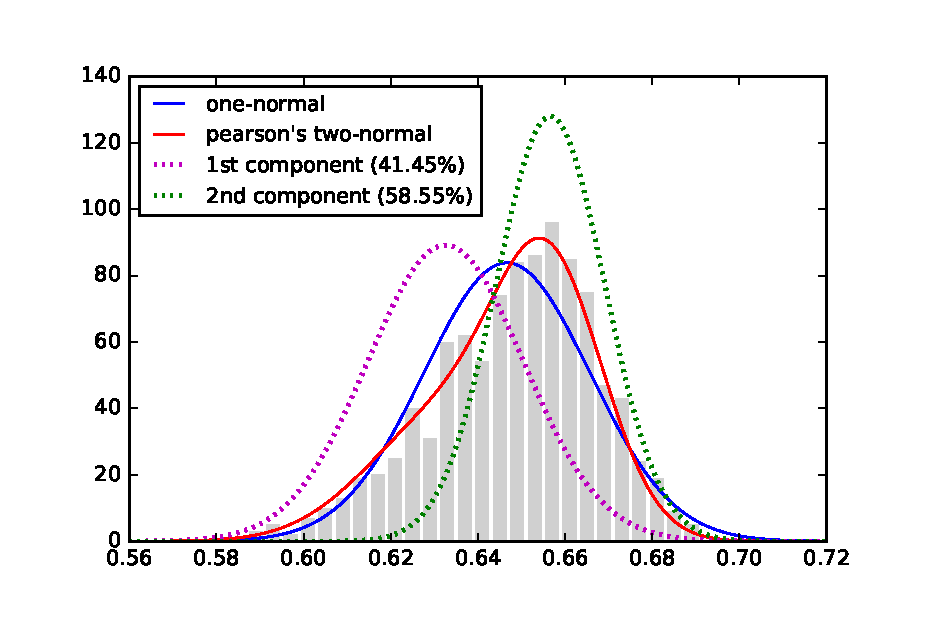
\includegraphics[width=0.8\linewidth]{figures/pearson-crab.eps}
  \caption{In this plot, the bar chart of the observations from Weldon is shown
    in grey. The blue solid line shows the single normal distribution fitting
    the data using Maximum Likelihood; And the solid line in red plots the
    mixture model of two normals distributions derived by Pearson using moment
    matching where its two components are also displayed in green and purple
    dotted lines.}
  \label{fig::pearson-crab}
  \end{subfigure}
  ~
  \begin{subfigure}[b]{0.95\textwidth}
  \centering
  \includegraphics[width=0.8\linewidth]{figures/pearson-crab-weibull.eps}
  \caption{Comparison between the Pearson's mixture of two normals and a single
    Weibull distribution. Pearson's mixture model provides a tighter fitting at
    the mode of empirical distribution. Note that the density function of
    Weibull distribution is much more complicated than that of normal
    distribution and it requires numeric means to estimate the parameters.}
  \label{fig::pearson-crab-weibull}
  \end{subfigure}
  \caption{Pearson's Mixture of Two Normals on ``Breadth of Forehead of Crabs''}
\end{figure}

Pearson used two normal distributions to fit the observations. He assumed that
the observed data are sampled from $\pi_1 \mathcal{N}(\mu_1, \sigma_1^2) + \pi_2
\mathcal{N}(\mu_2, \sigma_2^2),~(\pi_1 + \pi_2 = 1)$. To estimate the
parameters, namely, the means ($\mu_1, \mu_2$) and standard-variance ($\sigma_1,
\sigma_2$) of the two normal distributions as well as the proportions ($\pi_1,
\pi_2$) of the two components, Pearson followed the method of moments (which was
also introduced by himself in 1894). Though moment matching is superseded by
Fisher's method of maximum likelihood~\cite{pfanzagl1994parametric} in nowadays
classic statistical modelling, it was a relatively numerically simpler approach
in most cases. However, the calculation was still formidable and daunting at the
time without the aid of computer or other machinery of any kind.
Mathematically, the problem involves five parameters $\mu_1, \mu_2, \sigma_1,
\sigma_2$ and $\pi_1$ (since we can obtain $\pi_2 = 1 - \pi_1$) and to find a
solution, the parameters need to ensure that the mixture model matches on the
first five moments. Pearson derived a ninth degree polynomial (nonic) and two
candidate real roots are found. He finally chose the solution on the basis of
agreement with the sixth moment. In \Cref{fig::pearson-crab}, the dashed curve
in red shows Pearson's mixture and its two components are displayed in purple
and green dotted lines. Clearly, the mixture is skewed and better fits the
histogram than a single normal distribution. And indeed, two subspecies are
identified which verifies the hypothesis of Weldon.

It is quite an advanced idea to leverage latent variables for statistical
modeling at that time. Otherwise properly fitting the asymmetric observations
would involve a much more complicated distribution. In fact, we can also explain
the data with a skewed Weibull distribution, the parameter of which are
nevertheless computationally difficult to estimate (The Maximum Likelihood
estimator for the shape parameter is the solution to the equation $\frac{1}{k} =
\frac{\sum_{i=1}^N (x_i^k\log x_i - x_N^k \log x_N) }{\sum_{i=1}^N (x_i^k -
x_N^k)}- \frac{1}{N}\sum\limits_{i=1}^N \log x_i$, and numeric methods, which
were very primitive at the time of late 19th century, is required). Therefore
Weibull distribution was not a practical option for Pearson to fit the data when
the aid of computers was not available. In \Cref{fig::pearson-crab-weibull}, we
compare Peason's mixture of two normals with one single Weibull distribution
fitting the data using Maximum Likelihood. The difference between the two curves
is not significant. However, Pearson's result seems to fit better at the mode
around $0.66$.

\subsection{Mixture Models --- Development of the EM algorithm}

Although solving the mixture model with the method of moments is a very
laborious task and performing the necessary calculation is even more
heroic~\cite{mclachlan2004finite}, it does not always yield the optimal solution
in the statistical sense. The maximum likelihood approach, however, possesses
superior statistical property as it tries to place higher probability close to
the observed data and are more often unbiased. With the development of
optimization in the modern computer science, statistical modeling is able to
utilize numerical algorithms to solve Maximum Likelihood Estimation (MLE).
Among the different optimization methods, the Expectation-Maximization (EM)
algorithm~\cite{dempster1977maximum} has greatly stimulated interest in the use
of mixture models as well as other PLVMs. Several reasons can be accounted for
the popularisation of the EM algorithm: (1) It is generally easy to implement
the algorithm and it has virtually no parameters to tune, as compared to, for
example, gradient descent, where a carefully selected learning step is required
to ensure fast training; (2) It usually does not need any special treatment to
handle the constraints of the model. For example, in the normal mixture problem,
the standard-variance of a component normal is always positive. In the EM
algorithm, this is naturally satisfied since it is computed as the empirical
standard-variance of the complete data generated out of the posterior
distribution; (3) EM is a flexible family of approaches where the variational
distribution in the expectation step can be simplified (or constrained) for the
purpose of computation efficiency (e.g. mean-field EM and convex relaxations,
\cite[see][Chapter 5, 7]{wainwright2008graphical}) and the maximization step can
also be substituted by an ascend step. We leave the details of EM algorithm in
\Cref{sec::bg-em}. In this section, we provide a brief comparison between EM
algorithm and Pearson's method of moments and show how Pearson's result can be
improved by the EM algorithm.

\begin{figure}[ht!]
  \centering
  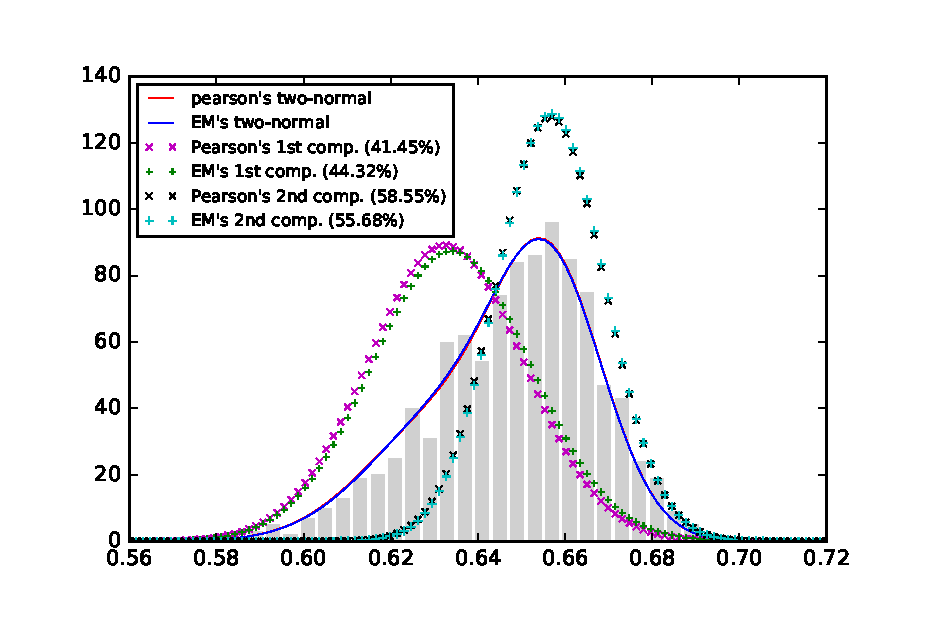
\includegraphics[width=0.8\linewidth]{figures/pearson-crab-em.eps}
  \caption{Comparison of the mixture model of two normals between Pearson's
  approach and EM algorithm. The two mixture models are very close to each
  other showing that the moment-matching method of Pearson obtains a near
  optimal likelihood.}
  \label{fig::pearson-crab-em}
\end{figure}

We plot the curves of the mixture models of the two methods as well as their
components in \Cref{fig::pearson-crab-em}. The results are almost
identical. To assess the quality of the model quantitatively, Pearson used the
Chi-square test~\cite{pearson1900x} which he proposed to examine if the observed
data is indeed from the model. We follow his practice and report the result in
\Cref{tab::pearson-em-crab}.

\begin{table}[h]
  \centering
  \caption{Pearson's Chi-square test and p-Value for a single normal model, a
    single Weibull model, and the two normal mixture model of Pearson and EM
    algorithm in the ``Breadth of Forehead of Crabs'' problem. For the normal
    models, we also include the model parameters.}
  \label{tab::pearson-em-crab}
  \setlength\tabcolsep{5pt}
  \begin{tabular}{c|cccccc|c|cc}
    Method & $\mu_1$ & $\mu_2$ & $\sigma_1$ & $\sigma_2$ & $\pi_1$ & $\pi_2$
           & freedom & Chi-square & p value \\ \hline \hline
    Single Normal & 0.6466 & \NA & 0.0190 & \NA & 1 & \NA & 2 & 71.6836 &
    \num{2.157e-6} \\
    Single Weibull & \NA & \NA & \NA & \NA & \NA & \NA &
    2 & 28.3841 & 0.2904 \\
    Pearson & 0.6326 & 0.6566 & 0.0179 & 0.0125 & 0.4145 & 0.5855 &
    5 & 21.0342 & 0.5186 \\
    EM & 0.6339 & 0.6568 & 0.0182 & 0.0124 & 0.4432 & 0.5568 &
    5 & 20.8438 & 0.5304 \\
    %\hline \hline
  \end{tabular}
\end{table}

As expected, we see that the EM algorithm results in the smallest Pearson's
Chi-square. In less mathematical terms, the observed data is distributed more
close to the model given by the EM algorithm. In addition, the p-values in the
significant test show that it is more certain that the data is sampled from the
mixture normal of EM algorithm. To an extent, the assessment on the Weldon's
crab dataset justifies the use of EM algorithm to solve MLE in applications of
mixture modeling.

% EM:         (statistic=20.843800910788627, pvalue=0.53040874121547321)
% Pearson:    (statistic=21.034210586530026, pvalue=0.51862468978687204)
% uni-normal: (statistic=71.683615393997414, pvalue=2.1571531876646807e-06)
% Pearson:    (0.6326, 0.6566, 0.0179, 0.0125, 0.4145, 0.5855)
% EM:         (0.6339, 0.6568, 0.0182, 0.0124, 0.4432, 0.5568)
% Weibull:    (statistic=28.384054004025337, pvalue=0.29047889023764795)

\subsection{From Mixture Models to Topic Modeling}

Since late 1990s, the study on document understanding has witnessed a new
approach of PLVMs which is often referred to as topic modeling. The first well
recognized topic modeling method, probabilistic latent semantic
indexing~(PLSI)~\cite{hofmann1999probabilistic}, is simple yet effective.
Essentially it sees the unigram word ($w_d$) distribution of a document $d$ as a
$K$-mixture of multinomial distributions $\beta_1, \dots, \beta_K$ with
proportions $\theta_{d, 1}, \dots, \theta_{d, k}$. Those $\beta_K$ are referred
to as ``topics'' because the words of large probabilities in a component are
often semantically related. In addition, the topic weights $\theta_d$ of a
document provides a succinct summary of the documents. Computationally,
$\theta_d$ has a much lower dimensionality than $w_d$ and thus can be leveraged
as a (part of) feature vector in tasks such as document classification or
clustering. Moreover, $\theta_d$ is semantically meaningful as the similarity of
$\theta_d$'s correlates with the similarity of the subject of documents, which
can be greatly useful in document understanding, information indexing, \etc.

In terms of modeling the latent variables, there are two milestone progresses:
the Bayesian inference and nonparametric statistics. The early efforts promoting
the Bayesian nonparametrics and advocating the theoretical formalization of
topic modeling, specifically, the analysis on random processes of exchangeable
partitions~\cite{pitman1995exchangeable}, are the lectures taught by
\citeauthor{pitman2002combinatorial} at Berkeley in Spring
\citeyear{pitman2002combinatorial}. Many results obtained in this
direction~\cite{blei2009topic,blei2003latent,blei2010nested} are immediate fruit
of the course and readers interested in a principle introduction on this topic
should refer to the lecture notes~\cite{pitman2002combinatorial} and the
references therein.

\emph{Bayesian inference} departs from the traditional MLE framework. It assumes
a prior distribution on latent variables parametrized by the
\emph{hyperparameters}. The advantages of introducing a prior on latent
variables are mainly two folds and we show them using the Latent Dirichlet
Allocation~(LDA)~\cite{blei2003latent} as an example: (1) It enables user to
incorporate human knowledge about the latent variables into modeling. In
document understanding, the word distribution of a topic as well as the
proportion of topics for a document are naturally \emph{sparse}. LDA encourages
such behavior by using a Dirichlet prior with a small hyperparameter $\valpha$.
(2) By selecting the form of prior distribution carefully, the prior and
posterior distributions can be in the \emph{same} family (with different
parameters though). Such conjugate prior-posterior pairs are computationally
beneficial in both Gibbs sampling as well as variational inference. LDA chooses
Dirichlet as the conjugate prior to the multinomial distribution, and the
posterior distribution is also a Dirichlet of parameter $\valpha + \mathbf{n}$,
where $\mathbf{n}$ is often referred as the pseudo-count of the latent variables
in each topic. Estimation method for Bayesian inference has also been greatly
developed beyond MLE. There are two major estimation methods of the latent
variables in Bayesian setting which are Bayesian Estimator (Posterior
Expectation) and Maximum a Posterior (MAP). The first computes the posterior
expectation of the latent variables given the observed data while the second
selects the value with the maximal probability in the posterior distribution,
which can be viewed as an extension of the MLE method. In the context of topic
modeling, it has been noticed that Bayesian estimator is more popular than MAP.
The major criticism of MAP is the fact that it is still a point estimation in
nature. Specifically in topic modeling, it is not uncommon that the posterior
distribution of the latent variables are in fact multi-modal. And therefore it
is computationally infeasible (or even intractable) to calculate MAP due to the
non-convex nature of the problem.

\emph{Nonparametric statistics} aims to model the data with possibly infinite
number of latent variables. In topic modeling, it implies that one can model a
infinite number of topics or words in the vocabulary. Although in practice it
does not seem to be immediately useful since there is always a finite
upper-bound for these quantities, it is critical to rely on expert knowledge to
appropriately select the values. Nonparametric statistics are most powerful to
adaptively learn the number of latent variables that are adequately large to
explain the data by using random processes. Random processes are extensively
studied in recent literature, as surveyed in \cite{hajek2015random}, including
Gaussian process~\cite{rasmussen2006gaussian}, Dirichlet
process~\cite{teh2011dirichlet}, Indian buffet
process~\cite{ghahramani2005infinite}, and hierarchical
processes~\cite{teh2012hierarchical,griffiths2004hierarchical,blei2010nested},
just to name a few. Mathematically, to model the latent variables from possibly
infinite number of choices, the nonparametric approach assumes a random process
as prior. Computationally, there are mainly two strategies, Gibbs sampling and
truncated variational inference, to estimate the posterior distribution of the
possibly infinite number of latent variables. Gibbs sampling takes advantage of
the fact that the prior process usually yields a simple prediction rule of one
latent variable given all others. For example, in Dirichlet process, using the
notion of Chinese restaurant process~\cite{pitman2002combinatorial}, the
probability of a latent variable choosing an existing value is proportional to
the number of other latent variables of the same value, or a new value
proportional to the hyperparameter $\alpha$:

\begin{align}
  \P_{CRP}(z_i = k | z_1, \dots, z_{i-1}, z_{i+1}, \dots, z_N)
    \propto
      \begin{cases}
        \sum\limits_{j = 1, j \neq i}^N \indct( z_j = k )
        & \text{if $k < K$} \\
        \alpha
        & \text{if $k = K + 1$}
      \end{cases}
\end{align}
%
where it is supposed that the value of $z_j, j \neq i$ is choosing from $1,
\dots, K$  and for any $k < K$ the support is nonempty. Therefore it is feasible
to investigate sampling methods for inference. While alternatively, another
strategy for estimation is to approximate the possibly infinite posterior with a
finite approximation. For the Dirichlet Process (as well as the generalized
Pitman-Yor two-parameter process~\cite{pitman1997two}), the truncating
approximation is based on a stick-breaking~\cite{ishwaran2011gibbs}
interpretation. It views the process as breaking a stick with the proportion as
a sample from a Beta distribution and the truncation stops the breaking after
there is a predefined number of sticks generated. Both of the above two
strategies have advantages: Gibbs sampling does not need to truncate the size of
latent variables by a finite number, while the truncated variational inference
is generally computational efficient. However, as shown in
\cite{wang2012truncation}, it is possible to combine the two ideas together by
performing the E-step in variational EM via sampling.

\section{Latent Variables for Optimization}

Previous research such as topic modeling mainly incorporates the latent
variables for the purpose of knowledge discovery. Another motivation to use
latent variable models is efficient computation. In previous discussion of the
``Breadth of Forehead of Crabs'' example, we have already seen that by
introducing latent variables, the mixture model is much easier to compute than
that of the Weibull distribution. However, contemporary efforts in the direction
of leveraging PLVMs for efficient computation was less explored. In one of our
recent work, Dual-Clustering Maximum Entropy (DCME)~\cite{wang2016dcme}, it is
demonstrated that PLVM is an effective means to improve the optimization
efficiency.

We explore PLVM in the context of Maximum Entropy (ME) models. ME is a classic
approach in classification as well as word embedding. However, it becomes
computationally challenging when the number of classes or the vocabulary size is
large. DCME approaches the problem by optimizing ME in its primal-dual form. The
key insight is to introduce a latent cluster assignment for each training
instance and assume that the dual variables of an instance are determined by the
corresponding latent assignment. As an initial investigation, we use the latent
variables in a much simpler manner than the mixture models. Specifically, we
restrict the latent variable to distribute as a Kronecker delta which has
support only on a single value, in contrast to the case of mixture models where
the latent variable is subject to a more general multinomial distribution. DCME
naturally leads to an approximation of the dual variables which can be computed
by a K-means like clustering. More importantly, it enables an efficient
online-offline computation scheme whose computational complexity does not
depends on the number of classes nor the vocabulary size. Empirical studies
demonstrated that DCME significantly outperforms state-of-the-art approaches.

\section{Contribution of this thesis}

In this thesis, I describe a range of applications where latent variables can be
leveraged for knowledge discovery and efficient optimization. Works in this
thesis demonstrate that PLVMs are a powerful tool for modelling incomplete
observations. Through incorporating latent variables and assuming that the
observations such as literature citations, pairwise preferences in crowdsourcing
as well as unstructured text are generated following tractable distributions
parametrized by the latent variables, PLVMs are flexible and effective to
discover knowledge in data mining problems, where the knowledge is
mathematically modelled as continuous or discrete values, distributions or
uncertainty. For example, when modelling literature citations, latent variables
can be inferred to identify research topics and evolution of research themes;
While only observing pairwise preferences labelled by non-expert workers in
crowdsourcing, PLVM as a generative process is capable to recover the ground
truth ranked lists; And finally, by fitting the unstructured text with
underlying phrasal structures, it can be shown that both the phrasal allocation
and phrase embeddings are effectively computed. In addition, I also explore the
PLVMs for deriving efficient algorithms. It has been shown that latent variables
can be employed as a means for model reduction or to facilitating
computation/sampling of intractable distributions. For instance, PLVM has been
shown to improve efficiency of Maximum Entropy which does not scale well as the
number of classes by performing model reduction with the latent variables; In
addition, in cases where the computation involves a intractable distribution,
latent variables are also investigated to facilitate the calculation via Gibbs
sampling.

\section{Overview of this Thesis}

In \Cref{chp::bg}, we briefly discuss a few key mathematical ingredients that
can greatly facilitate the understanding of PLVMs. Next, we move on to show two
scenarios where PLVMs are applied for knowledge discovery in \Cref{chp::clda}
and \Cref{chp::tpp}. Leveraging PLVMs for efficient optimization is presented in
\Cref{chp::dcme}. The last work we propose in this thesis takes the advantages
of PLVMs in both aspects, namely extracting the phrasal structure with an
efficient optimization scheme and effectively learning the semantic embeddings
of phrases, is discussed in \Cref{chp::plans}.

The first work analyzes the citations of
literatures~\cite{wang2013understanding}. Understanding how research themes
evolve over time in a research community is useful in many ways (e.g., revealing
important milestones and discovering emerging major research trends).  In this
study, we propose a novel way of analyzing literature citation to explore the
research topics and the theme evolution by modeling article citation relations
with a probabilistic generative model.  The key idea is to represent a research
paper by a ``bag of citations'' and model such a ``citation document'' with a
probabilistic topic model.  We explore the extension of a particular topic
model, i.e., Latent Dirichlet Allocation~(LDA), for citation analysis, and show
that such a Citation-LDA can facilitate discovering of individual research
topics as well as the theme evolution from multiple related topics, both of
which in turn lead to the construction of evolution graphs for characterizing
research themes.  We test the proposed citation-LDA on two datasets: the ACL
Anthology Network~(AAN) of natural language research literatures and PubMed
Central~(PMC) archive of biomedical and life sciences literatures, and
demonstrate that Citation-LDA can effectively discover the evolution of research
themes, with better formed topics than (conventional) Content-LDA.

The second work explores PLVMs in a crowdsourcing setting~\cite{wang2016tpp}.
Crowdsourcing services make it possible to collect huge amount of annotations
from less trained crowd workers in an inexpensive and efficient manner.
However, unlike making binary or pairwise judgements, labeling complex
structures such as ranked lists by crowd workers is subject to large variance
and low efficiency, mainly due to the huge labeling space and the annotators'
non-expert nature. Yet ranked lists offer the most informative knowledge for
training and testing in various data mining and information retrieval tasks such
as \textit{learning to rank}.  In this paper, we propose a novel generative
model called ``Thurstonian Pairwise Preference'' (\textsc{Tpp}) to infer the
true ranked list out of a collection of crowdsourced pairwise annotations.  The
key challenges that \textsc{Tpp} addresses are to resolve the inevitable
incompleteness and inconsistency of judgements, as well as to model variable
query difficulty and different labeling quality resulting from workers' domain
expertise and truthfulness.  Experimental results on both synthetic and
real-world datasets demonstrate that \textsc{Tpp} can effectively bind pairwise
preferences of the crowd into rankings and substantially outperforms previously
published methods.

Another aspect of PLVMs is to improve the efficiency of optimization. To this
end, we devote another chapter to discuss the study of Dual-Clustering Maximum
Entropy~\cite{wang2016dcme}.  Maximum Entropy (ME), as a general-purpose machine
learning model, has been successfully applied to various fields such as text
mining and natural language processing.  It has been used as a classification
technique and recently also applied to learn word embedding. ME establishes a
distribution of the exponential form over items (classes/words). When training
such a model, learning efficiency is guaranteed by \emph{globally} updating the
entire set of model parameters associated with \emph{all} items at \emph{each}
training instance. This creates a significant computational challenge when the
number of items is large. To achieve learning efficiency with affordable
computational cost, we propose an approach named Dual-Clustering Maximum Entropy
(DCME).  Exploiting the primal-dual form of ME, it conducts clustering in the
dual space and approximates each dual distribution by the corresponding cluster
center.  This naturally enables a hybrid online-offline optimization algorithm
whose time complexity per instance only scales as the product of the
feature/word vector dimensionality and the cluster number. Experimental studies
on text classification and word embedding learning demonstrate that DCME
effectively strikes a balance between training speed and model quality,
substantially outperforming state-of-the-art methods.

The last work presented in this thesis investigates PLVMs for learning phrasal
allocation. Existing word embedding methods are intrinsically hindered by its
unigram (bag-of-words) assumption of language. Although efforts towards
resolving the semantics for higher level of language units (\eg phrase,
sentence) have been made, most of them either rely on an external resource or
employ a complicated decoding algorithm for identifying the composition
structure. In this work, we propose an effective yet simple generic algorithm,
\PLANS{}~(PLANS), to compute the phrase embedding. We propose transient Chinese
Restaurant Process (tCRP) as a prior for words to allocate the phrases within
which they are enclosed. In addition, similar to Skipgram, PLANS estimates the
embedding for words/phrases with negative sampling.  Nevertheless the major
challenge in learning is that a reasonable size of the phrases need to be
carefully retained and less confident ones are constantly pruned during
training. PLANS address this with an online block algorithm which refreshes the
set of phrases based on their ``frequencies'' in the corpus periodically. In
addition, simulated annealing (SA) is applied in the sampling process to
stabilize the learned phrase set. Empirical study demonstrates that PLANS is
able to successfully (1) identify the frequent phrases in the dataset; and (2)
estimate their semantics. By applying the learned representation from PLANS to
NLP tasks such as sentiment and topical classification, we observe that the
phrase embedding significantly outperforms other standard features such as
bag-of-words, N-grams, as well as state-of-the-art word embedding.

\section{Background} \label{sec::dcme_review}

In this section, we first provide a brief review on Maximum Entropy (ME)
framework, together with a short account for the works on optimization of the
ME. Then we discuss current research development for extreme classification,
\ie, classification with a larger item number.

\subsection{Maximum Entropy Framework}

The general formulation of ME is simple. For a data instance $t$, ME establishes
a distribution over $N$ items:

\begin{equation}
  \P_t(i; \THETA) = \frac{\exp(f_t(i; \THETA))}
  {\sum\limits_{j=1}^{N}\exp(f_t(j; \THETA))}, \quad  i = 1, \dots, N.
  \label{eq::me}
\end{equation}

where $f_t(i; \THETA)$ is the scoring function with model parameters $\THETA$,
which quantifies the affinity between instance $t$ and item $i$\footnote{In the
context of energy-based models, $-f_t(i; \THETA)$ is often referred as the
energy function~\cite{bengio2003neural}.}. In this chapter, we investigate ME in
two settings, namely, multi-class classification and word embedding.

For $N$-class classification, the dataset $\mathcal{D}$ consists of a collection
of instances $\{(\vx_t, i_t)\}$ with $\vx_t$ being a $D$-dimensional feature
vector and $i_t$ a label chosen from items $1, \dots ,N$.  The model $\vW =
[\vw_1, \dots, \vw_N]$ is a $D \times N$ matrix which specifies the scoring
function as:

\begin{flalign}
  & \cc && f_t(j; \THETA) = f_t(j; \vW) = \vw_j^T \vx_t &
  \label{eq::scr_classification}
\end{flalign}

In the word embedding setting, we focus our discussion on the continuous
bag-of-words algorithm (CBOW)~\cite{mikolov2013efficient}, but the analysis
easily extends to other models. As a language modeling technique, it predicts
the target word from a vocabulary of size $N$ given its surrounding context. The
$t$-th training instance contains a stream of words $w_{t,-c}, w_{t,-(c-1)},
\dots, w_{t,0}, \dots, w_{t, c-1}, w_{t,c}$ with the target word $i_t =
w_{t,0}$. CBOW calculates the compatibility between the $j$-th word in the
vocabulary and the context as:

\begin{flalign}
  &\ee
  && f_t(j; \THETA) = f_{t}(j; \vV, \vH) = f(\vv_j, \vhb_t) = \vv_j^T \vhb_t &
  \nonumber \\
  &&& \textrm{where}\quad \vhb_t = \frac{1}{2c}
  \sum\limits_{-c \le p \le c, p \neq 0} \vh_{w_{t,p}} &
  \label{eq::scr_embedding}
\end{flalign}

The model parameters $\vV=[\vv_1, \dots, \vv_N]$ and $\vH=[\vh_1, \dots,
\vh_N]$ are two $D \times N$ matrices of the ``input'' and ``output'' vector
representations of words, respectively.

\subsection{Optimization of ME}

Various algorithms for ME have been studied in the literature. They approach the
optimization by solving either the primal or the dual problem. The primal form
maximizes the log-likelihood of the dataset. Methods of this direction, as
surveyed in \cite{malouf2002comparison,yuan2012recent}, include iterative
scaling algorithms~\cite{berger1996maximum,darroch1972generalized}, coordinate
descent~\cite{huang2010iterative}, stochastic gradient
descent~\cite{tsuruoka2009stochastic} and Quasi-Newton
method~\cite{gao2007comparative}, just to name a few. Their training complexity
per instance is $\oo(DN)$. This is a consequence of having to enumerate
\emph{all} items when computing the probability of a single item or the
corresponding gradient. On the other hand, another line of research tackles the
problem by maximizing the entropy of \emph{dual distributions}.  Constraint
optimization techniques, such as exponentiated
gradient~\cite{collins2008exponentiated} and dual coordinate
descent~\cite{yu2011dual}, are investigated. Since the dimensionality of dual
distributions is in fact the same as the number of items, their training
complexity is still linear in $N$. Consequently, all these algorithms are
impractical with large numbers of items due to the prohibitively expensive
computational cost.

\subsection{Learning with Large Item Number}

Scaling algorithms for learning when the number of items $N$ is large have
become a recent research direction with focus on maintaining the training
complexity sublinear in $N$.  Among them, hierarchical approaches explore a
taxonomy (of items) and convert the problem into a series of binary predictions
along the tree branches, which potentially reduces the complexity from $\oo(N)$
to $\oo(\log N)$. Though efforts have been made in large multi-class (extreme)
classification~\cite{choromanska2015logarithmic,choromanska2013extreme} and word
embedding~\cite{morin2005hierarchical,mnih2009scalable,mikolov2013efficient},
finding balanced tree structures that provide an effective partition of items is
difficult by itself, and thus their use is limited in practice. Another work of
extreme classification, \cite{YenHRZD16}, has developed a fast active set
algorithm for max-margin classifiers by exploiting the sparsity of feature
vectors. The training speed-up, nevertheless, is generally insignificant for
dense data representations such as word embeddings. To the best of our
knowledge, the most effective approaches for training ME models with a large $N$
are sampling-based methods, for instance \cite{bengio2008adaptive}, offering a
trade-off between speed and precision. In addition, as pointed out by
\cite{mnih2012fast}, noise-contrastive estimation (NCE)~\cite{gutmann2010noise}
is regarded as the state-of-the-art sampling algorithm which employs the idea of
``learning by comparison'': It reduces the $N$-item ME problem to a binary
classification between samples from the training data and ``noise'' from the
proposal distribution, and is guaranteed to converge to the solution of ME. Yet
in practice, a slightly simpler variant, negative sampling
(NS)~\cite{mikolov2013distributed}, is proposed to train CBOW and skip-gram
though mathematically it does not solve ME. However, one drawback is that
algorithms of this kind inevitably suffer from sampling variance. More
crucially, the computational efficiency is gained at the expense of only
updating the model parameters associated with the sampled items, while the due
change of the rest is discarded. Learning efficiency is therefore sacrificed.

% In contrast, the proposed DCME can achieve much better learning efficiency while
% maintaining a computational cost comparable to these sampling-based methods.

\section{\DCME{}}\label{sec::dcme_dcme}

In this section, we present a \DCME{}~(DCME) approach which has two advantages
regarding learning and computational efficiency: (1) The model parameters
associated with \emph{all} items are updated at \emph{each} training instance;
and (2) The time complexity is independent of $N$.

\subsection{Primal-dual ME}

Different from existing approaches, DCME solves the ME problem in a primal-dual
fashion. Suppose that the dataset $\mathcal{D}$ has $M$ instances and $N$ items
where the $t$-th instance selects the $i_t$-th item. We start the derivation
from the primal ME formulation which maximizes the log-likelihood:

\begin{alignat}{-1}
  \sum\limits_{t=1}^M \log(\P_t(i_t; \THETA))=&
  \sum\limits_{t=1}^M \big(  f_t(i_t; \THETA)
  - \log \sum\limits_{j=1}^N \exp f_t(j; \THETA) \big) \nonumber\\
  =& \sum\limits_{t=1}^M \big(  f_t(i_t; \THETA) - A_t(\THETA) \big)
\label{eq::primal_ll}
\end{alignat}

where $A_t(\THETA)$ is referred to as the log-partition function and its
conjugate dual is revealed by the following
lemma~\cite{hiriart1993convex,wainwright2008graphical}:

\begin{lem}\label{lem::conj_dual}
  Assume $ \P(i; \vs) = \exp(s_i) / \sum\limits_{j=1}^N \exp(s_j)$
  and $A(\vs) = \log \sum\limits_{j = 1}^N \exp(s_j)$,
  the conjugate duality between the log-partition function and negative entropy
  states:

  \begin{align}
    A(\vs) &= \max\limits_{\vmu \in \Delta_N}
                    \{ \sum\limits_{j=1}^N \mu_j s_j -
                       \sum\limits_{j=1}^N \mu_j \log \mu_j \} \nonumber \\
           &= \max\limits_{\vmu \in \Delta_N}
                    \{ \E_{\vmu} [s_j] + \entropy(\vmu) \} \label{eq::conj_dual}
  \end{align}

  where the simplex set
  $\Delta_N = \{\mathbf{p} \in \mathbb{R}^{N}:
  p_j \ge 0, \sum\limits_{j=1}^N p_j = 1\}$

  and the maximizer is attained at:

  \begin{align}
    \mu_j^* = \P(j; \vs), \quad 1 \le j \le N \label{eq::conj_dual_sol}
  \end{align}

\end{lem}

\begin{proof}
  We use the following equivalence:
  \begin{align*}
    \E_{\vmu}[s_j] + \entropy(\vmu)
      &= -\sum\limits_{j=1}^N \mu_j \log \frac{\mu_j }{ \P(j; \vs) } +
          \log\sum\limits_{j=1}^N \exp(s_j) \nonumber \\
      &= -D_{KL}(\vmu || \P) + A(\vs)
  \end{align*}
where $D_{KL}(\vmu || \P)$ is the Kullback-Leibler (KL) divergence and note
$D_{KL}(\vmu || P) \ge 0$ and  $D_{KL}(P || P) = 0$. It follows that
$\vmu^* = \argmin\limits_{\vmu \in \Delta_N} D_{KL}(\vmu || P) = P$.
\end{proof}

In view of \Cref{lem::conj_dual}, we arrive at the primal-dual form of ME:

\begin{equation}
  \max\limits_\THETA
  \min\limits_{\substack{\vmu_t \in \Delta_N \\ 1 \le t \le M}}
  \sum\limits_{t=1}^M \big( f_t(i_t; \THETA) - \E_{\vmu_t}[f_t(j;\THETA)] -
  \entropy(\vmu_t) \big) \label{eq::me_primal_dual}
\end{equation}

where $\vmu_t$ is the \emph{dual distribution} for instance $t$.

\subsection{Dual Distribution Clustering}

\Cref{lem::conj_dual} implies that $\vmu_t^*$ is determined by $f_t(j;\THETA)$.
In less mathematical terms, similar instances choose similar items (in
probabilities). As real-world data instances generally possess a clustering
structure instead of being randomly distributed, it is expected that dual
distributions also form clusters. For the text classification example of venue
prediction, if papers are grouped by topics, those in the same group should have
similar chance of getting published at a particular venue; For learning word
embedding, we anticipate contexts of similar semantics yield target word
distributions that can be clustered together.

It is worth exploring the cluster structure of dual distributions to reduce
complexity. DCME rests on the idea of ``approximation by clustering'': By
clustering the dual distributions into $K$ groups, each $\vmu_t$ is assigned to
a cluster $c_t \in \{1, \dots K\}$, and is then approximated by the
corresponding \emph{cluster center} $\valpha_{c_t}\in\Delta_N$ which best
represents the group. The optimization problem of DCME can thus be formulated
as:

\begin{alignat}{-1}
  &\textrm{DCME:} && \qquad
\max\limits_\THETA
\min\limits_{\substack{\valpha_k \in \Delta_N \\ 1 \le k \le K}}
\min\limits_{\substack{1 \le c_t \le K \\ 1 \le t \le M}}
\sum\limits_{t=1}^M Q_t(\valpha_{c_t}; \THETA) \label{eq::dcme} \\
  &\textrm{where~~} &&
Q_t(\valpha_{c_t}; \THETA) =
  f_t(i_t;\THETA) -
  \E_{\valpha_{c_t}}[f_t(j;\THETA)] -
  \entropy(\valpha_{c_t})\big) \nonumber
\end{alignat}

\subsection{Online-Offline Optimization}

We employ Gauss-Seidel coordinate descent to solve \Cref{eq::dcme}.  Three
blocks of variables, namely, the model parameters $\THETA$, the cluster centers
$\{\valpha_k\}$, and the instances' cluster assignments $\{c_t\}$, are
successively updated while keeping others constant. In particular, we devise a
hybrid online-offline algorithm which breaks the computational bottleneck and
leads to a time complexity that only scales as $\oo(DK)$, as opposed to
$\oo(DN)$ in conventional ME algorithms.

\subsubsection{Updating cluster assignments~(Online)}

DCME approximates $\vmu_t$ by $\valpha_{c_t}$, and the cluster assignment $c_t$
is solved by:

\begin{equation}
  \argmin\limits_{1 \le k \le K} - \E_{\valpha_{k}}[f_t(j;\THETA)]
        - \entropy(\valpha_{k}) \label{eq::clu_mem}
\end{equation}

However, a na\"{i}ve computation would cost $\oo(DN + KN)$ time. It takes
$\oo(D)$ to evaluate $f_t(j;\THETA)$ for every item $1 \le j \le N$\footnote{In
  word embedding, one can compute the scoring function in $\oo(D)$ time. Note
  that the \emph{asymptotic} complexity of computing $\vhb_t$ in \emph{every}
sliding windows is $\oo(D)$ (independent of window size) with the sum $\sum_{-c
\le p \le c} \vh_{w_{t,p}}$ maintained by adding the new word and subtracting
the past word.}; For each cluster, another $\oo(N)$ is required to calculate
$\E_{\valpha_{k}}[f_t(j;\THETA)]$ and $\entropy(\valpha_k)$ by enumeration.

Fortunately, when the scoring function is linear in the feature/context vector,
the cost can be reduced to $\oo(DK)$ per instance. To see this, from
\eqref{eq::scr_classification} and \eqref{eq::scr_embedding} we have:

\begin{alignat}{-1}
  &\cc &
  \E_{\valpha_{k}}[f_t(j; \vW)] &= (\vW \valpha_{k})^T \vx_t
  \label{eq::exp_classification}\\
  &\ee &
  \E_{\valpha_{k}}[f_t(j; \vV,\vH)] &= (\vV \valpha_{k})^T \vhb_t
  \label{eq::exp_embedding}
\end{alignat}

The trick we apply here \emph{trades memory for time}: By storing $\vW
\valpha_{k}$, $\vV \valpha_{k}$ and $\entropy(\valpha_k)$ for $K$ clusters in
the offline update, it is merely a $D$-dimensional dot product to calculate
\Cref{eq::exp_classification} and \Cref{eq::exp_embedding}, and therefore the
cost to online update $c_t$ by \Cref{eq::clu_mem} is $\oo(DK)$.

\subsubsection{Updating cluster centers~(Offline)}

We update the cluster center $\valpha_k$ as well as the cached $\vW
\valpha_{k}$, $\vV \valpha_{k}$ and $\entropy(\valpha_k)$ only in the offline
computation. Let $\ii_k$ denote the index set of instances in the $k$-th
cluster, $\valpha_k$ satisfies:

\begin{align}
   \argmin\limits_{\valpha \in \Delta_N}
   -\E_{\valpha}\Bigg[\frac{1}{|\ii_k|}
                      \sum\limits_{t \in \ii_k}f_t(j; \THETA)\Bigg]
   -\entropy(\valpha) \label{eq::up_clu_center_opt}
\end{align}

Invoking \Cref{lem::conj_dual} again, \Cref{eq::up_clu_center_opt} has the
following closed-form solution:

\begin{align}
  \alpha_{k, j} = \frac{1}{Z} \exp\big(
      \frac{1}{| \ii_k |}
      \sum\limits_{t \in \ii_k} f_t(j;\THETA) \big)
  \label{eq::up_clu_center}
\end{align}

where a normalization term $Z$ is applied to keep $\sum\limits_{j=1}^N
\alpha_{k,j} = 1$. By the linearity of $f_t(j;\THETA)$, we express
\Cref{eq::up_clu_center} as:

\begin{alignat}{-1}
  &\cc & \quad
  \alpha_{k, j} = \frac{1}{Z} \exp\Big( \vw_j^T
  \frac{1}{| \ii_k |} \sum\limits_{t \in \ii_k} \vx_t\Big)
  \label{eq::up_clu_center_classification}\\
  &\ee &
  \alpha_{k, j} = \frac{1}{Z} \exp\Big( \vv_j^T
  \frac{1}{| \ii_k |} \sum\limits_{t \in \ii_k} \vhb_t\Big)
  \label{eq::up_clu_center_embedding}
\end{alignat}

which computes $\valpha_k$ with $\oo(D |\ii_k|  + D N)$ cost. In addition, it
takes $\oo(DN)$ and $\oo(N)$ to update $\vW \valpha_{k}$, $\vV \valpha_{k}$ and
$\entropy(\valpha_k)$, respectively. By choosing the interval between
consecutive offline updates such that $|\ii_k| = \beta N$ for a constant $\beta$
(1 for example), we obtain an average time complexity of $\oo(D)$ per instance.

\subsubsection{Updating model parameters~(Online/Offline)}

To optimize $\THETA$ with subgradient descent:

\begin{alignat}{-1}
  &\cc &
  \frac{\partial Q_t}{\partial \vw_j} &=
    \underbrace{\mathds{1}[i_t = j]\, \vx_t}_{(a)} +
    \underbrace{(-\alpha_{c_t, j} \vx_t)}_{(b)}
    \label{eq::mdl_upd_classification}\\
  &\ee &
  \frac{\partial Q_t}{\partial \vv_j} &=
    \overbrace{\mathds{1}[i_t = j]\, \vhb_t} +
    \overbrace{(-\alpha_{c_t, j} \vhb_t)}
    \label{eq::mdl_upd_embedding_v}\\
  &&
  \frac{\partial Q_t}{\partial \vh_{w_p^{(t)}}} &=
    \frac{1}{2c} (\vv_{i_t} - \vV \valpha_{c_t})
    \label{eq::mdl_upd_embedding_h}\\
  &&
  \textrm{for all}\; &-c \le p \le c,\; p \ne 0 \nonumber
\end{alignat}

where $\mathds{1}[i_t = j]$ is the indicator function which evaluates to 1 when
$i_t = j$ and 0 otherwise. In the following, we devise a hybrid
\emph{online-offline algorithm} which has an average expense of $\oo(D)$ time
per instance.

First, Term (a) in \Cref{eq::mdl_upd_classification} and
\Cref{eq::mdl_upd_embedding_v} only changes the model parameters associated with
the correct item $i_t$, namely $\vw_{i_t}$ and $\vv_{i_t}$, and can be updated
online in $\oo(D)$ time. Similarly, for word embedding
\Cref{eq::mdl_upd_embedding_h}, $\partial Q_t / \partial \vH$ can also be
updated online with $\oo(D)$ cost by keeping track of the sum of $\partial Q_t /
\partial \vh_{w}$ for all overlapping instances using a sliding window
technique.

Second, Term (b) in \Cref{eq::mdl_upd_classification} and
\Cref{eq::mdl_upd_embedding_v} changes the model parameters of all $N$ items.
We make two crucial observations here: (1) Term (b) of different items share the
\emph{same} direction $-\vx_t$ (or $-\vhb_t$); and (2) The scale vector
$\valpha_{c_t}$ \emph{only} depends on the cluster assignment $c_t$, but not the
individual instance $t$. Thus it is logical to perform offline update of Term
(b). The computation is postponed until $|\ii_{c_t}|$ is large enough, and then
Term (b) is calculated for all items $1 \le j \le N$ and instances $t \in
\ii_{c_t}$. Such ``lazy'' computation yields a total cost of $\oo(D |\ii_{c_t}|
+ D N)$, and we achieve an average $\oo(D)$ expense per instance if we wait
until $|\ii_{c_t}| \ge \beta N$.

\subsubsection{Tuning online/offline computation}

The overall complexity per instance is $\oo(DK)$ time, which is appealing as it
does not hinge on $N$.  Nevertheless, an inherent limitation in learning is the
delay of computing Term (b) until $|\ii_k| \ge \beta N$ in
\Cref{eq::mdl_upd_classification} and \Cref{eq::mdl_upd_embedding_v} ,
especially for items with large values $\alpha_{k, j}$. A heuristic improvement
we find effective in practice tunes the computation between online and offline
updates. By sorting items (using a heap) with decreasing $\alpha_{k,j}$, Term
(b) of the top $Q$ items are updated online while the others are updated
offline. The resulting average cost per instance becomes $\oo(D K + D Q + \log
Q)$. Computational efficiency is preferred with a small $Q$ while the priority
shifts to learning efficiency with a large $Q$.

\section{DCME Algorithm}\label{sec::dcme_algo}

We have already presented the DCME algorithm in previous section. In the
following, we first give an overview about the DCME algorithm, and then
illustrate its connections with K-means algorithm and the Dual ME respectively.

\subsection{Overall Procedures}

We summarize the learning procedure of DCME in \Cref{alg::dcme}. DCME assigns
each training instance $t$ to a dual cluster $c_t$ and performs the online model
update. Once the size of a dual cluster reaches $\beta N$, an offline model
update as well as the update of the dual cluster center are applied.  Although
the algorithm has a similar complexity as the sampling-based approaches such as
noise contrastive estimation~(NCE) and negative sampling~(NS), DCME allows the
\emph{entire} model to learn from \emph{every} training instance. In other
words, the model parameters associated with all items get updated when a new
training instance arrives, which yields superior performance over existing
methods, as will be shown in the experimental study.

\begin{algorithm}[h]
\caption{DCME algorithm}\label{alg::dcme}
  % \SetAlgoNoLine
  \KwIn{$M$ instances, a constant $\beta$, cluster number $K$, and top item
        number $Q$}
	\KwOut{Model $\mathbf{\THETA}$}
  Initialize $K$ clusters $\{\valpha_k\}$ \;
	\While{$\THETA$ is not optimal}{
    \begin{itemize}
      \item[--] Select an index $t$ from $\{1, \dots, M\}$
      \item[--] Find the cluster assignment $c_t$ by \eqref{eq::clu_mem}
      \item[--] Perform online update of Term (a) (and Term (b) of the \\
                 top $Q$ items) in \eqref{eq::mdl_upd_classification} (or
                \eqref{eq::mdl_upd_embedding_v}). For embedding, also \\
                update $H$ by \eqref{eq::mdl_upd_embedding_h}.
      \item[--] Add $t$ to $\ii_{c_t}$; \\
                if $|\ii_{c_t}| \ge \beta N$
        \begin{itemize}
          \item[--] Perform offline update of Term (b) in
                    \eqref{eq::mdl_upd_classification} (or
                    \eqref{eq::mdl_upd_embedding_v}).
          \item[--] Update cluster center $\alpha_{c_t}$ and empty
                    $\ii_{c_t}$
        \end{itemize}
    \end{itemize}
	}
\end{algorithm}

\subsection{Connection with K-means}

So far, readers might have already been aware of the resemblance between the
dual distribution clustering and the K-means algorithm. The following theorem
formally proves their connection:

\begin{thm}
  The dual distribution clustering in DCME is a generalized K-means
  algorithm using KL-divergence as the distance measurement in the simplex.
  Moreover, it converges as fast as K-means.
\end{thm}
\begin{proof}
  Using \Cref{lem::conj_dual}, the dual clustering satisfies:

  \begin{alignat}{-1}
    \min\limits_{\substack{\valpha_k\in \Delta_N ,  1 \le k \le K \\
                           1 \le c_t \le K , 1 \le t \le M}} \;
  \sum\limits_{t=1}^M D_{KL}(\valpha_{c_t} || P_t) \label{eq::k-means_clustering}
  \end{alignat}

  which minimizes the \emph{within-cluster KL-divergence} between
  $\valpha_{c_t}$ and $P_t$. It is the same minimization objective as K-means
  except that DCME measures the distance in the simplex space with
  KL-divergence\footnote{Technically, KL-divergence is not a true metric of
  distance.}. To illustrate this, notice that the dual clustering proceeds by
  alternating between the following two steps (See \Cref{fig::dual_cluster}):

\begin{itemize}
\item[--] Update $c_t = \argmin_{k} D_{KL}(\valpha_k || P_t)$, and $t$ is
  assigned to the cluster whose center is nearest to $P_t$ by KL-divergence.
\item[--] Update $\valpha_k = \argmin_{\valpha} \sum_{t \in \ii_k} D_{KL}(
  \valpha || P_t)$ where the cluster center is found as the point in the simplex
  with the least within-cluster distance.
\end{itemize}

General convergence results for the subgradient methods can be applied.
Specifically, the above two-step algorithm converges to the local minimum of the
problem \eqref{eq::k-means_clustering} as fast as the K-means
algorithm~\cite{bottou1995convergence},
\end{proof}

\begin{figure}[h!]
  \centering
  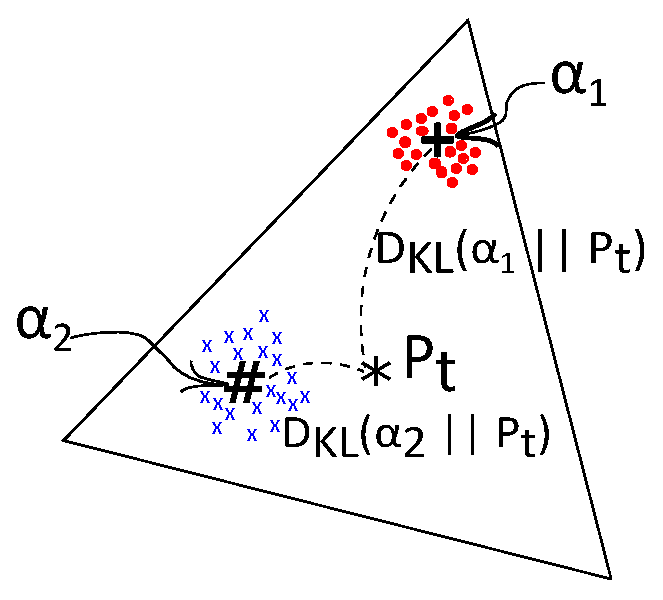
\includegraphics[width=0.4\linewidth]{dcme/dual_cluster_color.eps}
  \caption{Dual Clustering in the Simplex with KL-divergence}
  \label{fig::dual_cluster}
\end{figure}

\subsection{Connection with Dual ME}

The DCME is reminiscent of the dual ME, and we show the following results in the
classification setting:

\begin{thm} The dual form of DCME in classification is:
  \begin{align}
    \max\limits_{\substack{\valpha_k \in \Delta_N ,  1 \le k \le K \\
                           1 \le c_t \le K , 1 \le t \le M}}
                 &\qquad
    \sum\limits_{t=1}^M \entropy(\valpha_{c_t}) \label{eq::dual_dcme_op} \\
    \subjto \quad
    & \sum\limits_{t = 1}^M \mathds{1}[i_t = j]\; \vx_t =
    \sum\limits_{t = 1}^M \alpha_{c_t, j} \vx_t,~~ 1 \le j \le N \nonumber
  \end{align}
\end{thm}

The proof is omitted because it is very similar to the derivation of dual ME.
However, the dual form of DCME provides us with intuition of how DCME works: To
approximate $P_t$, the cluster center is restricted to reproduce the observed
statistics. Comparing it with the dual ME where $\vmu_t$ is in place of
$\valpha_{c_t}$, we see that the dual DCME has more restricted constraints. A
limiting case that DCME becomes identical to ME is when $K=M$, \ie{} each
instance is a singleton cluster with the only member being itself.

\section{Experiments}\label{sec::dcme_experiments}

We conduct experiments on tasks of text classification and word embedding,
evaluating the proposed DCME approach by examining its computational and
learning efficiency. For comparison, we implement two sampling-based approaches,
noise contrastive estimation~(NCE) and negative sampling~(NS), as well as the
maximum likelihood estimation using gradient descent~(GD). In order for DCME and
the sampling-based approaches to have comparable training speed, we set both the
cluster number $K$ of DCME and the sampling number of NCE and NS to 20, and also
control the interval between offline updates in DCME with $\beta = 1$. Two
variants of DCME, DCME-Q0 and DCME-Q10, are developed, the latter of which
applies the online/offline tuning with $Q=10$. All the algorithms are run with
20 threads in parallel on a 64-bit Linux machine with the Intel Xeon 3.60GHz CPU
(20 core). Our code is implemented in C and available for download at:
\url{https://www.dropbox.com/s/e6b3fj2w0lq6jbt/code.tar.gz}

\begin{figure*}
  \centering
        \begin{subfigure}[h]{0.7\textwidth}
            \centering
            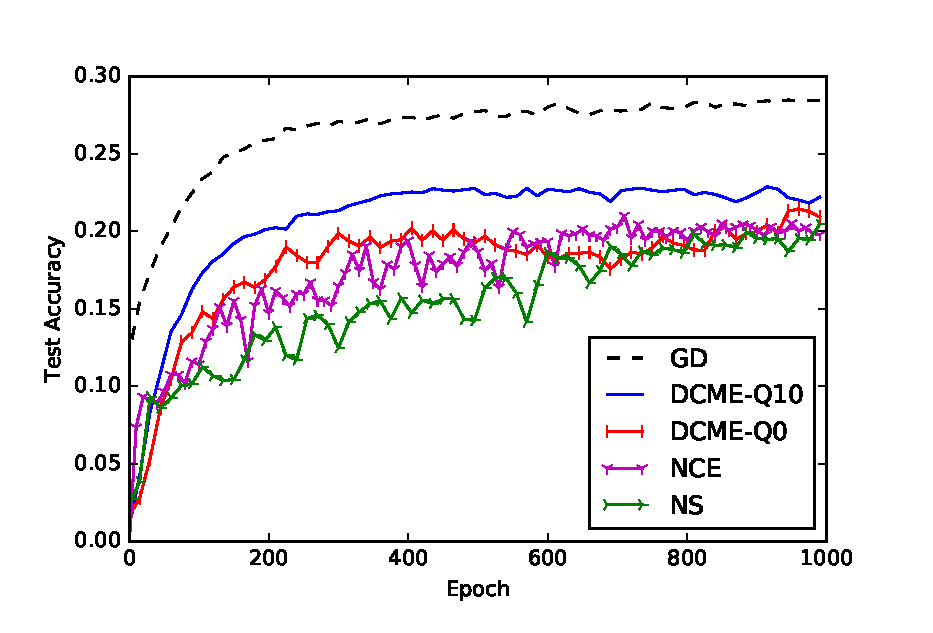
\includegraphics[width=\linewidth]{dcme/classification.eps}
            \captionsetup{justification=centering}
            \caption{Comparison of Test Accuracy for Classification\\
              Trained on ACM Digital Library Dataset}
            \label{fig::classification}
        \end{subfigure}
        \hfill
        \begin{subfigure}[h]{0.7\textwidth}
            \centering
            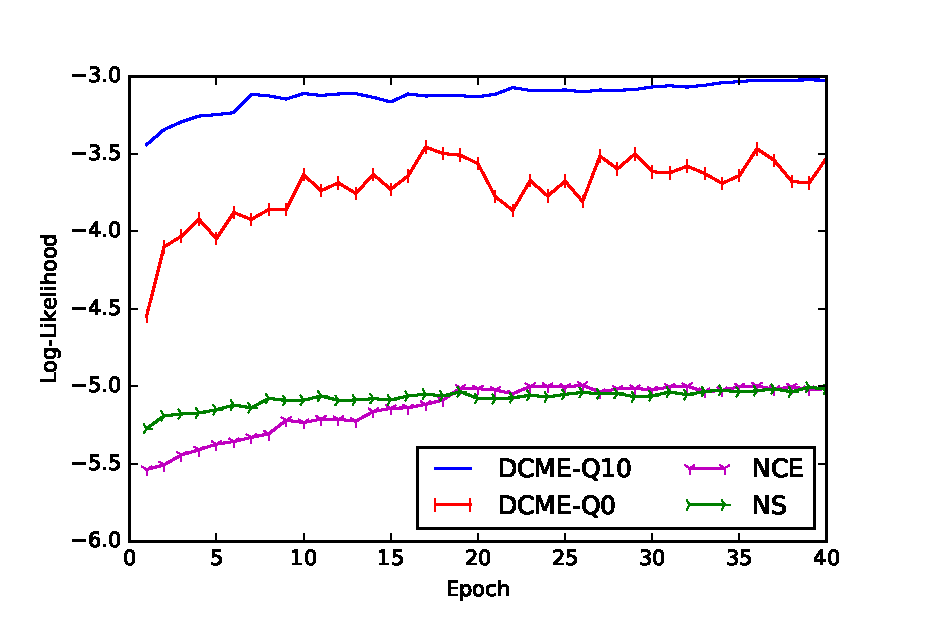
\includegraphics[width=\linewidth]{dcme/word_embedding.eps}
            \captionsetup{justification=centering}
            \caption{Comparison of Log-Likelihood for Embedding \\
              Trained on NYT Dataset}
            \label{fig::word_embedding}
        \end{subfigure}
        \begin{subfigure}[h]{0.65\textwidth}
            \centering
            \begin{tabular}{c|c|c|c|c}
              DCME-Q10  & DCME-Q0   & NCE   & NS        & GD     \\ \hline\hline
              9.50      & 7.94      & 6.21  & 6.16      & 165.91 \\
            \end{tabular}
            \captionsetup{justification=centering}
            \caption{Time Cost (Second) per Epoch in Classification}
            \label{tab::classification_time}
        \end{subfigure}
        \begin{subfigure}[h]{0.65\textwidth}
            \centering
            \begin{tabular}{c|c|c|c}
              DCME-Q10  & DCME-Q0   & NCE     & NS       \\ \hline\hline
              33.49     & 25.59     & 22.22   & 20.80    \\
            \end{tabular}
            \captionsetup{justification=centering}
            \caption{Time Cost (Minute) per Epoch in Embedding}
            \label{tab::we_time}
        \end{subfigure}
        \caption{ Performance on Text Classification and Word Embedding }
\end{figure*}

\subsection{Evaluation on Text Classification}

We employ the ME model to predict the publishing venue of research papers using
the abstract. A public dataset ACM Digital Library is investigated. It has
$162,460$ papers published at $1,236$ conferences. We hold out $10\%$ of the
documents for testing. Each paper is represented by the word count features of
the top $30,000$ frequent words.

\Cref{fig::classification} shows the learning curves of algorithms trained
at each epoch, and \Cref{tab::classification_time} reports the training
speed. It is clear that GD does not scale well to large number (thousands or
more) of items. DCME is 17-20 times faster than GD while the ratio is around 26
for sampling-based approaches. But it does give an estimation about the
upper-bound performance by leveraging the exact gradient information.  The curve
of GD converges in the least number of iterations while the test accuracy is the
highest.

DCME, on the other hand, achieves a computational efficiency similar to that of
the sampling-based approaches, but the accuracy is considerably higher.
Particularly, \Cref{fig::classification} validates that DCME benefits from
tuning the computation between online and offline updates. When $Q=10$, more
model parameters are updated online and there is thus less delay than that of
DCME-Q0. We also note that NCE and NS produce larger variances, which is
expected due to their sampling nature.

\subsection{Evaluation on Word Embedding}

For the word embedding task, we explore the New York Times (NYT) corpus from the
English Gigaword (Fifth Edition). It has a total of 1.35 billion words with
10.84 million unique terms. We retain the top 1 million frequent terms in the
vocabulary. To assess the performance, a randomly sampled \SI{1e-4} of the text
is withheld for testing. We train the word embeddings using CBOW with a context
window size of 10 and embedding dimensionality of 100.

We plot the test set average log-likelihood of each epoch in
\Cref{fig::word_embedding}, and report the time-per-epoch statistics in
\Cref{tab::we_time}. We do not evaluate GD in word embedding as it takes more
than days to run one epoch. The time costs for other algorithms are similar. The
results show that DCME remarkably outperforms NCE and NS.  However, DCME-Q0
exhibits a large performance variance. One possible explanation is as follows.
For $N$ as large as 1 million, the interval between offline updates is so long
that it creates two undesirable effects: (1) The delay results in a biased model
which contributes to a large training error; (2) The offline computation changes
the model drastically, as measured by the norm of the model difference, causing
inconsistency when another thread accesses the model while the offline update is
still in progress\footnote{The model parameters are shared by all threads and
  there is no mutex locks on writing to the model, which is a common practice
for efficiency in implementations including word2vec
  (\url{https://code.google.com/p/word2vec/}) and ours.}. For DCME-Q10, minimal
  variance is observed. Indeed, it offers the best trade-off between learning
  and computational efficiency.

\begin{table}[h]
  \centering
  \begin{tabular}{c||l|l|l}
    Model     & Semantic          & Syntactic         & Overall          \\
    \hline\hline
    DCME-Q10  & $\mathbf{-8.676}$ & $-8.648$          & $\mathbf{-8.654}$ \\
    DCME-Q0   & $-8.712$          & $\mathbf{-8.647}$ & $-8.663$          \\
    NCE       & $-8.784$          & $-8.782$          & $-8.783$          \\
    NS        & $-8.765$          & $-8.679$          & $-8.699$          \\
  \end{tabular}
  \captionsetup{justification=centering}
  \caption{Log-Likelihood on Semantic-Syntactic Word Relationship Dataset}
  \label{tab::we_analogy}
\end{table}

To assess the quality of the trained embeddings, we use the word analogy task,
which examines whether the embeddings learn the semantic/syntactic relationships
of words. For instance, the question which word is similar to ``small'' in the
same sense as ``biggest'' to ``big'' can be solved by predicting the target word
with a context vector $\vh_{biggest} - \vh_{big} + \vh_{small}$. We evaluate the
trained word embeddings after 15 epochs. And the results on the
Semantic-Syntactic Word Relationship test set~\cite{mikolov2013efficient} are
summarized in \Cref{tab::we_analogy}, where the best performance is highlighted
in bold. Again, it confirms that DCME achieves better model quality than
sampling-based NCE and NS.

% since they represent the main state of the art methods that can work efficiently with large numbers of items for ME.

% 0.017287 %   Semantic accuracy: 0.016449 %   Syntactic accuracy: 0.017556 %
% 0.017426 %   Semantic accuracy: 0.017061 %   Syntactic accuracy: 0.017543 %
% 0.016231 %   Semantic accuracy: 0.015777 %   Syntactic accuracy: 0.016377 %
% w2v
% 0.016666 %   Semantic accuracy: 0.015606 %   Syntactic accuracy: 0.017006 %
% 0.015336 %   Semantic accuracy: 0.015305 %   Syntactic accuracy: 0.015346 %
% 0.015792 %   Semantic accuracy: 0.015731 %   Syntactic accuracy: 0.015811 %

\section{Conclusions}\label{sec::dcme_conclusion}

We propose a novel optimization method, \DCME{}~(DCME), which solves the Maximum
Entropy problem in its primal-dual form. Although it has a similar complexity as
the sampling-based approaches, it allows the entire model to learn from every
training instance, which we believe is the first algorithm that is efficient
both in learning and computation. DCME exploits the dual clustering and
approximates dual distributions by cluster centers. It maintains an affordable
complexity using a hybrid online-offline optimization algorithm. Empirical
studies demonstrate that DCME outperforms state-of-the-art algorithms such as
NCE and NS in learning tasks with large numbers of items. A promising future
research direction is to investigate the nonparametric mixture models for dual
clustering. By taking advantages of probabilistic latent cluster assignments and
learning the number of clusters from the data, we expect a better approximation
for dual distributions.


\newpage
\bibliographystyle{aaai}
\bibliography{refs}


\end{document}
